\begin{figure}[!ht]
 \centering
 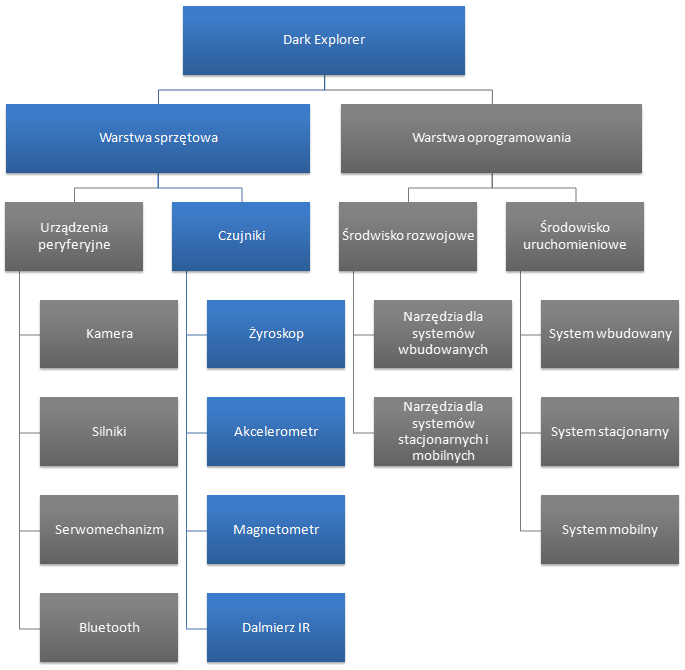
\includegraphics[height=125mm]{../images/ch04/dark_explorer_platform_hardware.png}
 \caption{Struktura platformy robota mobilnego po zakończeniu prac. Kolorem oznaczono zakres prac opisanych w bierzącym rozdziale.}
 \label{fig:DarkExplorerPlatformHardware}
\end{figure}

\section{Inercjalny system nawigacyjny}
W celu rozwinięcia możliwości robota, zamontowano w nim elementy przy pomocy
których, została podjęta próba stworzenia inercjalnego systemu nawigacyjnego
(INS\footnote{Inertial Navigation System}). Założeniem było, aby robot mobilny
zapamiętał tor ruchu po jakim się porusza, gdy jest niesiony na ręce
osoby operującej nim. Następnie na podstawie wykonanych pomiarów robot miał
powrócić po zapamiętanym torze w miejsce początkowe. Poniższy rozdział omawia
pokrótce czym jest INS, opisuje zasadę działania jego elementów oraz sposób
wykorzystania tych podzespołów do osiągnięcia wystarczająco dobrych efektów.

\subsection{Wprowadzenie do INS}
% http://citeseerx.ist.psu.edu/viewdoc/download?doi=10.1.1.63.7402&rep=rep1&type=pdf


Inercjalny system nawigacyjny jest to narzędzie służące do określenia położenia,
prędkości oraz orientacji obiektu w przestrzeni, bez korzystania z żadnych
zewnętrznych elementów naprowadzających, które byłyby dla niego punktem
odniesienia. Wykorzystuje on jedynie elementy wbudowane, składające się na
inercjalną jednostkę pomiarową (IMU\footnote{Inertial Measurement Unit}).
\begin{figure}[!ht]
 \centering
 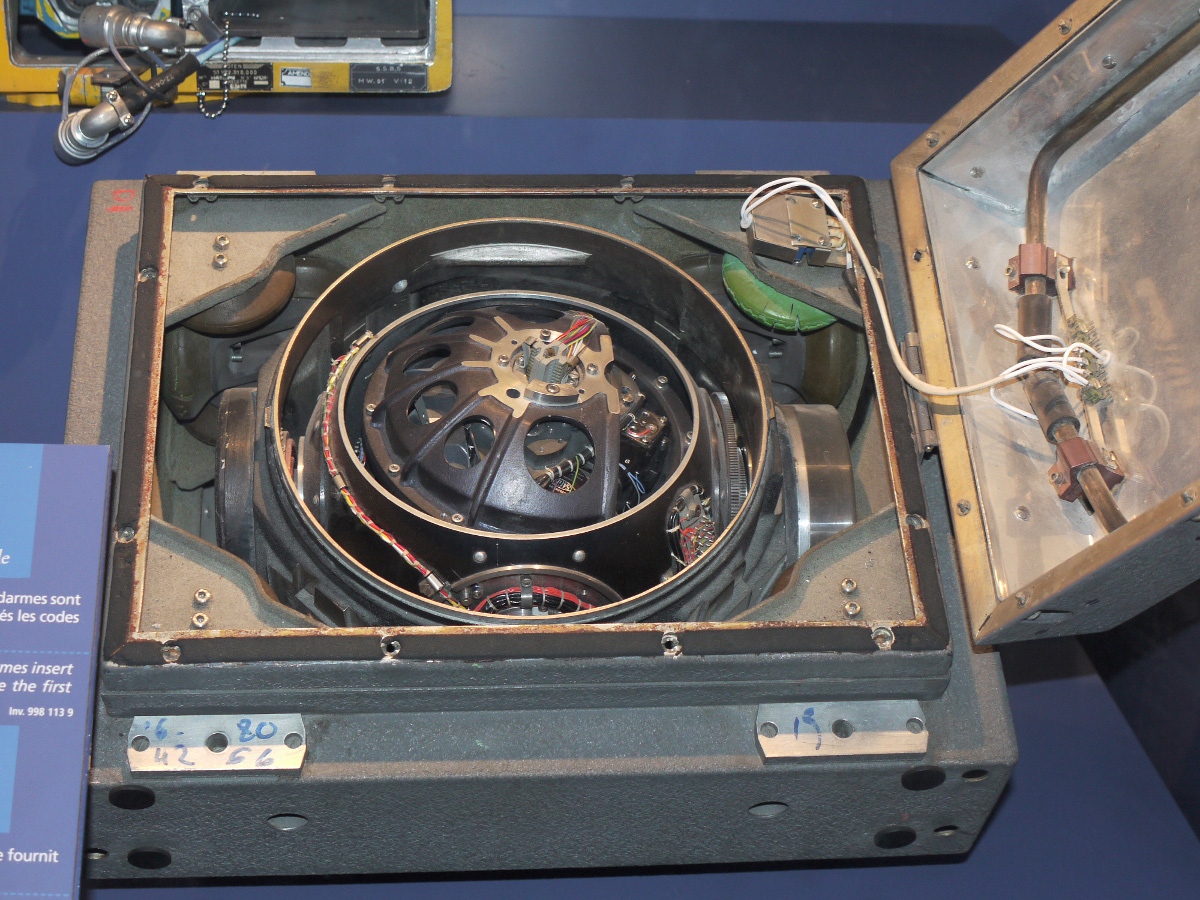
\includegraphics[height=100mm]{../images/ch04/INS-zdjecie.jpg}
 \caption[INS francuskiego IRBM S3]{INS francuskiego IRBM S3\footnotemark}
 \label{fig:Zyrokompas}
\end{figure}
\footnotetext{źródło: \url{http://en.wikipedia.org/wiki/Inertial_navigation_system}}

Inercjalne systemy nawigacyjne mają zastosowanie tam, gdzie jest potrzebna
informacja o aktualnym położeniu obiektów, natomiast nie ma możliwości odbioru
sygnału zewnętrznego, wymaganego do działania takich urządzeń jak na przykład urządzeń GPS. 
Systemy tego typu są stosowane w: samolotach, statkach, łodziach podwodnych, pojazdach
bezzałogowych czy statkach kosmicznych. Pierwsze rozwiązania tego typu były drogie i bazowały na bardzo
dużych gabarytowo elementach mechanicznych. 
\begin{figure}[!ht]
 \centering
 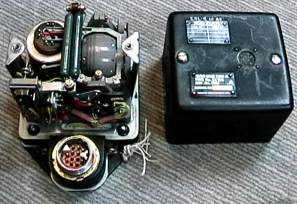
\includegraphics[height=50mm]{../images/ch04/gyrocompass.jpg}
 \caption[Żyrokompas samolotowy]{Żyrokompas samolotowy\footnotemark}
 \label{fig:Zyrokompas}
\end{figure}
\footnotetext{źródło: \url{http://www.gyroscopes.org/uses.asp}}

Rozwój miniaturowych układów elektromechanicznych MEMS\footnote{Microelectromechanical Systems} otworzył przed nami cały
wachlarz potencjalnych nowych zastosowań INS, np. do śledzenia ruchów ludzi bądź
zwierząt.

\begin{figure}[!ht]
 \centering
 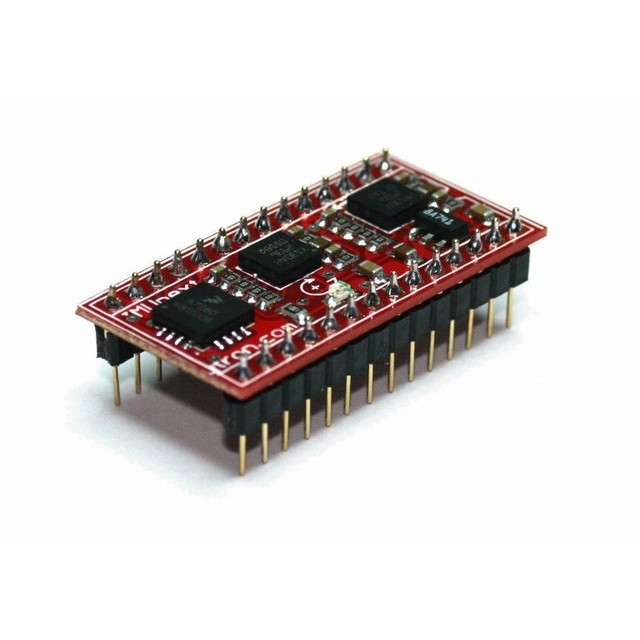
\includegraphics[height=50mm]{../images/ch04/mems_imu.jpg}
 \caption[IMU stworzone przy pomocy układów MEMS]{IMU stworzone przy pomocy układów MEMS, cena ok.: 80\$\footnotemark}
 \label{fig:Zyrokompas}
\end{figure}
\footnotetext{źródło: http://www.flytron.com}

\subsection{Elementy IMU robota}
System nawigacyjny o którym mowa w tym rozdziale oblicza swoje położenie na
podstawie ciągłego badania przyspieszenia liniowego oraz prędkości kątowej. INS
musi otrzymać na starcie wartości początkowe położenia oraz prędkości z jaką się
porusza, aby móc zacząć wyznaczać dalsze przemieszczenie i zmiany w orientacji.

Robot mobilny został wyposażony w IMU składające się z następujących elementów MEMS:
\begin{itemize}
  \item cyfrowy żyroskop trójosiowy L3G4200D firmy STMicroelectronics
  \item analogowy akcelerometr trójosiowy MMA7260 firmy Freescale
  \item cyfrowy magnetometr dwuosiowy firmy MMC2120MG firmy Memsic
\end{itemize}
Elementy użyte do wykonania IMU zostały wybrane pod kątem walorów ekonomicznych. 
Nie były przeprowadzane testy porównawcze pomiędzy podzespołami danego typu.
Zasada działania poszczególnych elementów oraz opis ich wykorzystania można znaleźć w kolejnych podrozdziałach.
